\newpage
\chapter{Coordinate Transformations}

% \localtableofcontents*

\newpage

\section{Constructing Transformation Matrix}

\subsection{Rotation Matrix}

From: \href{https://mathworld.wolfram.com/RotationMatrix.html}{wolfram}

\begin{enumerate}
    \item 2-D (in $\mathbb{R}^{2}$):

        Rotating an object to a new coordinate system:

        \begin{figure}[ht]
            \centering
            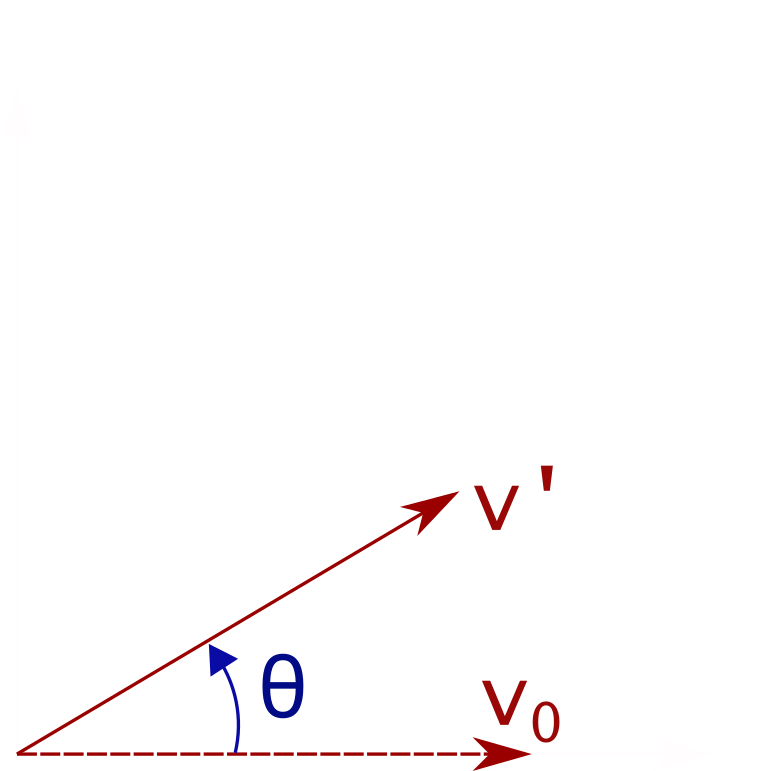
\includegraphics[width=0.35\textwidth]{img/RotationMatrix_1000}
            \caption{Rotating object}
            \label{fig:RotationMatrix_1000-png}
        \end{figure}

        In $\mathbb{R}^{2}$, consider the matrix that rotates a given
        vector $\mathbf{v}_{0}$ by a counterclockwise angle $\theta$ in
        a fixed coordinate system. Then

        \begin{equation}
            \mathbf{T}_{\theta} = \begin{bmatrix}
                \cos \theta & -\sin \theta \\
                \sin \theta & \cos \theta
            \end{bmatrix}
        ,\end{equation}

        so

        \begin{equation}
            \mathbf{v}^{'} = \mathbf{T}_{\theta}\mathbf{v}_{0}
        .\end{equation}

        \begin{figure}[ht]
            \centering
            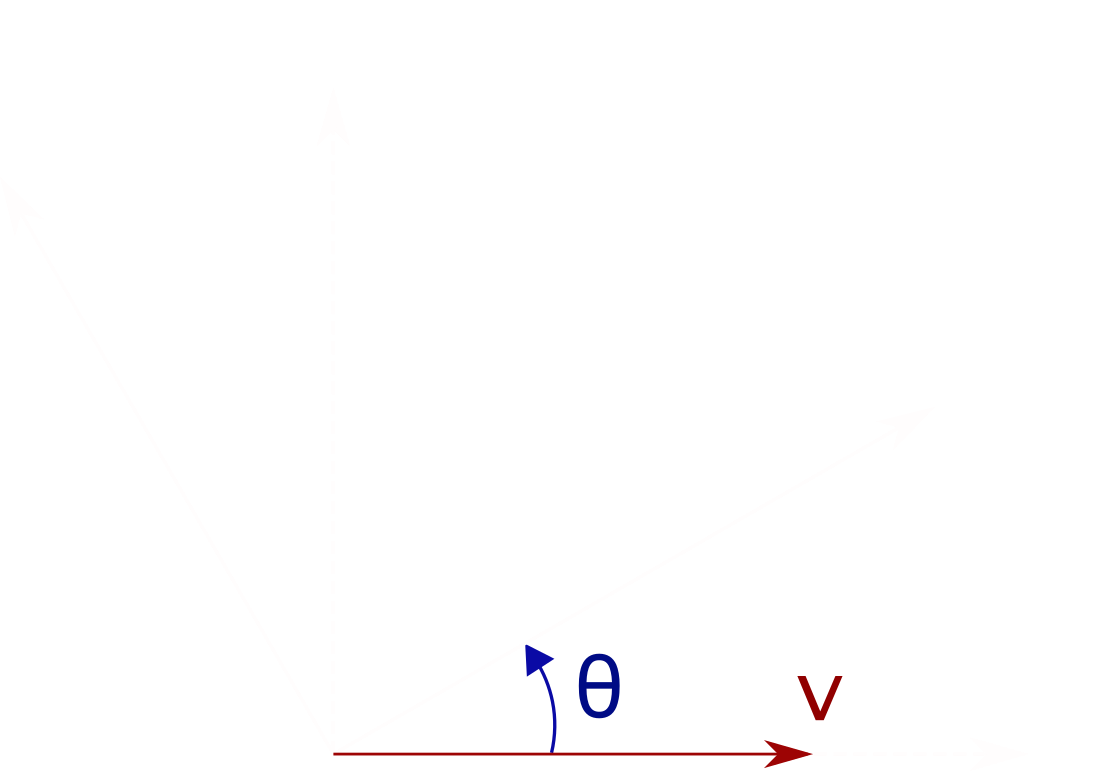
\includegraphics[width=0.5\textwidth]{img/RotationMatrixAxes_1000}
            \caption{Rotating Axes}
            \label{fig:RotationMatrixAxes_1000-png}
        \end{figure}

        On the other hand, consider the matrix that rotates the
        \textit{coordinate system} through a counterclockwise angle $\theta$.
        The coordinates of the fixed vector $\mathbf{v}$ in the rotated
        coordinate system are now given by a rotation matrix which is the
        \textit{transpose} of the fixed-axis matrix, as can be seen on the
        second figure, is equivalent to rotating the vector by
        a counterclockwise angle $-\theta$ relative to a fixed set of axes,
        giving:

        \begin{equation}
            \mathbf{T}_{\theta}^{'} = \begin{bmatrix}
                \cos \theta & \sin \theta \\
                -\sin \theta & \cos \theta
            \end{bmatrix}
        .\end{equation}

        This is the convention commonly used in textbooks.

    \item 3-D ($\mathbb{R}^{3}$):

        In $\mathbb{R}^{3}$, coordinate system rotations of the
        \textit{x-}, \textit{y-} and \textit{z-axis} in a counterclockwise
        direction when looking towards the origin give the matrices:

        \begin{equation}
            \mathbf{R}_{x}(\varphi) =
            \begin{bmatrix}
                1 & 0 & 0 \\
                0 & \cos \varphi & \sin \varphi \\
                0 & -\sin \varphi & \cos \varphi
            \end{bmatrix}
        .\end{equation}

        \begin{equation}
            \mathbf{R}_{y}(\theta) =
            \begin{bmatrix}
                \cos \theta & 0 & -\sin \theta \\
                0 & 1 & 0 \\
                \sin \theta & 0 & \cos \theta
            \end{bmatrix}
        .\end{equation}

        \begin{equation}
            \mathbf{R}_{z}(\psi) =
            \begin{bmatrix}
                \cos \psi & \sin \psi & 0 \\
                -\sin \psi & \cos \psi & 0 \\
                0 & 0 & 1
            \end{bmatrix}
        .\end{equation}

        Any \textbf{rotation} can be given as a composition of rotations
        about three axes (\textbf{Euler's rotation theorem}), and thus
        be represented by a $3 \times 3$ matrix operating on a vector.

        \begin{equation}
            \begin{bmatrix}
                x_{1}^{'} \\ x_{2}^{'} \\ x_{3}^{'}
            \end{bmatrix}
            =
            \begin{bmatrix}
                t_{11} & t_{12} & t_{13} \\
                t_{21} & t_{22} & t_{23} \\
                t_{31} & t_{32} & t_{33}
            \end{bmatrix}
            \begin{bmatrix}
                x_{1} \\ x_{2} \\ x_{3}
            \end{bmatrix}
        .\end{equation}

    \item \textbf{Euler's angles of XYZ rotation:}

        With the order of \textit{xyz} rotation the rotation matrix is
        composed as:

        \begin{equation}
            \scalebox{0.85}{
                $ \begin{array}{ll}
                    \mathbf{T}
                    &= \mathbf{R}_{z}(\psi)\mathbf{R}_{y}(\theta)\mathbf{R}_{x}(\varphi) \\
                    &=
                    \begin{bmatrix}
                        \cos \psi & \sin \psi & 0 \\
                        -\sin \psi & \cos \psi & 0 \\
                        0 & 0 & 1
                    \end{bmatrix}
                    \begin{bmatrix}
                        \cos \theta & 0 & -\sin \theta \\
                        0 & 1 & 0 \\
                        \sin \theta & 0 & \cos \theta
                    \end{bmatrix}
                    \begin{bmatrix}
                        1 & 0 & 0 \\
                        0 & \cos \varphi & \sin \varphi \\
                        0 & -\sin \varphi & \cos \varphi
                    \end{bmatrix} \\
                    &=
                    \begin{bmatrix}
                        \cos \theta \cos \psi
                        & \cos \psi \sin \theta \sin \varphi - \cos \varphi \sin \psi
                        & \cos \varphi \cos \psi \sin \theta + \sin \varphi \sin \psi \\
                        \cos \theta \sin \psi
                        & \cos \varphi \cos \psi + \sin \theta \sin \varphi \sin \psi
                        & \cos \varphi \sin \theta \sin \psi - \cos \psi \sin \varphi \\
                        -\sin \theta
                        & \cos \theta \sin \varphi
                        & \cos \theta \cos \varphi
                    \end{bmatrix}
                \end{array} $
            }
        \end{equation}

        Then the three \textit{Euler angles} for a \textit{xyz} rotation
        can be obtained:

        \begin{equation}
            \varphi = \atantwo(t_{32}, t_{33})
        ,\end{equation}

        \begin{equation}
            \theta = \atantwo \left(-t_{31}, \sqrt{ t_{32}^{2} + t_{33}^{2}} \right)
        ,\end{equation}

        \begin{equation}
            \psi = \atantwo(t_{21}, t_{11})
        ,\end{equation}

        where $\atantwo(y, x)$ definition is:

        \begin{equation}
            \atantwo(y, x) = \left\{
                \begin{array}{ll}
                    \arctan\left(\frac{y}{x}\right) & if \quad (x > 0),\\
                    \arctan\left(\frac{y}{x}\right) + \pi & if \quad (x < 0) \land (y \ge 0),\\
                    \arctan\left(\frac{y}{x}\right) - \pi & if \quad (x < 0) \land  (y < 0),\\
                    \frac{\pi}{2} & if \quad (x = 0) \land  (y > 0),\\
                    -\frac{\pi}{2} & if \quad (x = 0) \land  (y < 0),\\
                    undefined & if \quad (x = 0) \land (y = 0)
                \end{array}
            \right\}
        .\end{equation}

        \textbf{Note} the angle limitation for values returned while doing
        an Euler angle decomposition of a \textbf{rotation} matrix:

        \begin{equation}
            \begin{array}{l}
                \varphi \in (-\pi, \pi) \\
                \theta \in (-\frac{\pi}{2}, \frac{\pi}{2}) \\
                \psi \in (-\pi, \pi)
            \end{array}
        .\end{equation}

    \item Euler's angles of \textbf{ZYX} rotation:

        For a rotation defined in \textit{zyx} order the rotation matrix is:

        \begin{equation}
            \scalebox{0.85}{
                $ \begin{array}{ll}
                    \mathbf{T}
                    &= \mathbf{R}_{x}(\varphi)\mathbf{R}_{y}(\theta)\mathbf{R}_{z}(\psi) \\
                    &=
                    \begin{bmatrix}
                        1 & 0 & 0 \\
                        0 & \cos \varphi & \sin \varphi \\
                        0 & -\sin \varphi & \cos \varphi
                    \end{bmatrix}
                    \begin{bmatrix}
                        \cos \theta & 0 & -\sin \theta \\
                        0 & 1 & 0 \\
                        \sin \theta & 0 & \cos \theta
                    \end{bmatrix}
                    \begin{bmatrix}
                        \cos \psi & \sin \psi & 0 \\
                        -\sin \psi & \cos \psi & 0 \\
                        0 & 0 & 1
                    \end{bmatrix} \\
                    &=
                    \begin{bmatrix}
                        \cos \theta \cos \varphi
                        & - \cos \theta \sin \varphi
                        & \sin \varphi \\
                        \cos \psi \sin \varphi + \cos \varphi \sin \theta \sin \psi
                        & \cos \varphi \cos \psi - \sin \theta \sin \varphi \sin \psi
                        & -\cos \theta \sin \psi \\
                        \sin \varphi \sin \psi - \cos \varphi \cos \psi \sin \theta
                        & \cos \psi \sin \theta \sin \varphi + \cos \varphi \sin \psi
                        & \cos \theta \cos \psi
                    \end{bmatrix}
                \end{array} $
            }
        .\end{equation}

        \textbf{Note that the angles $\varphi$, $\theta$ and $\psi$ defined here are
        different from the \textit{XYZ} rotation defined above!} The rotation
        is performed by first rotating around \textit{z-axis} counterclockwise
        by an angle $\psi$, then around \textit{y-axis} counterclockwise
        by an angle $\theta$ and finaly around \textit{x-axis}, counterclockwise,
        by an angle $\varphi$.

        Then the \textit{Euler's angles} can be obtained as:

        \begin{equation}
            \left\{ \begin{array}{l}
                \varphi = \arctan \left( \frac{-t_{12}}{t_{11}} \right)\\
                \theta = \arcsin \left( t_{13} \right) \\
                \psi = \arctan \left( \frac{-t_{23}}{t_{33}} \right)
            \end{array} \right.
        .\end{equation}


    \item Alternate way of constructing \textbf{Rotation matrix} without specifying
        angles:

        The rotation matrix to a new coordinate system can be constructed from
        its axes, where the rotation matrix can be defined as:

        \begin{equation}
            \mathbf{T}_{R} = \begin{bmatrix}
                x_1 & x_2 & x_3 \\
                y_1 & y_2 & y_3 \\
                z_1 & z_2 & z_3 \\
            \end{bmatrix}
        ,\end{equation}

        where $\mathbf{x} = [x_1, x_2, x_3]^{T}$, $\mathbf{y} = [y_1, y_2, y_3]^{T}$
        and  $\mathbf{z} = [z_1, z_2, z_3]^{T}$ are unit vectors in the direction
        of \textit{x-}, \textit{y-} and \textit{z-axis} of the new coordinate
        system.


        \begin{bbox}[0.85]
            The \textbf{transformation matrix} can be defined by any two vectors
            $\mathbf{u}$ and $\mathbf{v}$, where $\mathbf{u}$ defines the direction
            of \textit{x-axis} and $\mathbf{v}$ defines the \textit{xy-plane}.
            To construct the \textbf{rotation matrix} use the following steps:

            \begin{enumerate}
                \item create x-axis of unit lenght

                    \begin{equation}
                        \mathbf{x} = \frac{\mathbf{u}}{||\mathbf{u}||}
                    .\end{equation}

                \item create z-axis of unit lenght

                    \begin{equation}
                        \mathbf{z}
                        = \frac{\mathbf{u} \times \mathbf{v}}{||\mathbf{u} \times \mathbf{v}||}
                    .\end{equation}

                \item create y-axis of unit lenght

                    \begin{equation}
                        \mathbf{y}
                        = \frac{\mathbf{z} \times \mathbf{x}}{||\mathbf{z} \times \mathbf{x}||}
                    .\end{equation}

                \item compose \textbf{rotation matrix}

                    \begin{equation}
                        \mathbf{T}_{R} = \begin{bmatrix}
                            \mathbf{x}^{T} \\
                            \mathbf{y}^{T} \\
                            \mathbf{z}^{T}
                        \end{bmatrix}
                    .\end{equation}
            \end{enumerate}

            The creation of the \textbf{rotation matrix} by any two other vectors is
            analogic, as \textbf{orthogonal} base must be constructed first, then
            the matrix is composed of its vectors.
        \end{bbox}

        \begin{bbox}[0.85]

            To test, whether the transformation matrix is correct, one can use
            the orthogonality criterion:

            \begin{equation}
                \mathbf{T}^{T} = \mathbf{T}^{-1}
            \end{equation}

            \begin{equation}
                \mathbf{T}\mathbf{T}^{T} = \mathbf{T}^{T}\mathbf{T} = \mathbf{I}
            \end{equation}

            or

            \begin{equation}
                \det(\mathbf{T}) = 1
            \end{equation}

        \end{bbox}

\end{enumerate}


\section{Coordinate Transformation}

\begin{itemize}
    \item \textbf{Rotation:}

        Let $\mathbf{A}^{T} = [a_{x}, a_{y}, a_{z}]$ be the original coordinates,
        $\mathbf{B}^{T} = [b_{x}, b_{y}, b_{z}]$ be the transformed coordinates, and
        $\mathbf{T}$ a tranformation matrix in the form:

        \begin{equation}
            \mathbf{T} = \begin{bmatrix}
                x_1 & x_2 & x_3 \\
                y_1 & y_2 & y_3 \\
                z_1 & z_2 & z_3
            \end{bmatrix} = \begin{bmatrix}
                \mathbf{x} \\
                \mathbf{y} \\
                \mathbf{z}
            \end{bmatrix}
        ,\end{equation}

        where $\mathbf{x} = [x_1, x_2, x_3]$, $\mathbf{y} = [y_1, y_2, y_3]$ and
        $\mathbf{z} = [z_1, z_2, z_3]$ are the \textit{x-axis}, \textit{y-axis} and
        \textit{z-axis} \textbf{unit vectors}, respectively, of the new coordinate
        system defined in the original one, while sharing their origin.

        The following applies:

        \begin{equation}
            \mathbf{T} \times \mathbf{A} = \mathbf{B}
        ,\end{equation}

        and

        \begin{equation}
            \mathbf{T}^{T} \times \mathbf{B} = \mathbf{A}
        .\end{equation}

        \textbf{Note:} Perpendicular vector is  created using \textit{cross-product}.
\end{itemize}


\section{Tensor Transformation}

From:
\href{https://wp.optics.arizona.edu/optomech/wp-content/uploads/sites/53/2016/10/OPTI_222_W21.pdf}{source 1},
\href{https://www.continuummechanics.org/principalstressesandstrains.html}{source 2},
\href{https://www.ecourses.ou.edu/cgi-bin/eBook.cgi?doc=&topic=me&chap_sec=07.2&page=theory}{source 3}

Let real symmetric matrix  $\mathbf{A}$ be the original tensor,
real symmetric matrix $\mathbf{B}$ the transformed tensor, and
orthogonal matrix $\mathbf{T}$ a tranformation matrix in the form:

\begin{equation}
    \mathbf{A} = \begin{bmatrix}
        \sigma^{A}_{11} & \sigma^{A}_{12} & \sigma^{A}_{13} \\
        \sigma^{A}_{21} & \sigma^{A}_{22} & \sigma^{A}_{23} \\
        \sigma^{A}_{31} & \sigma^{A}_{32} & \sigma^{A}_{33}
    \end{bmatrix}
,\end{equation}

\begin{equation}
    \mathbf{B} = \begin{bmatrix}
        \sigma^{B}_{11} & \sigma^{B}_{12} & \sigma^{B}_{13} \\
        \sigma^{B}_{21} & \sigma^{B}_{22} & \sigma^{B}_{23} \\
        \sigma^{B}_{31} & \sigma^{B}_{32} & \sigma^{B}_{33}
    \end{bmatrix}
,\end{equation}

\begin{equation}
    \mathbf{T} = \begin{bmatrix}
        x_1 & x_2 & x_3 \\
        y_1 & y_2 & y_3 \\
        z_1 & z_2 & z_3
    \end{bmatrix} = \begin{bmatrix}
        \mathbf{x} \\
        \mathbf{y} \\
        \mathbf{z}
    \end{bmatrix}
,\end{equation}

where $\mathbf{x} = [x_1, x_2, x_3]$, $\mathbf{y} = [y_1, y_2, y_3]$ and
$\mathbf{z} = [z_1, z_2, z_3]$ are the \textit{x-axis}, \textit{y-axis} and
\textit{z-axis} \textbf{unit vectors}, respectively, of the new coordinate
system defined in the original one, while sharing their origin.

The transformation matrix $\mathbf{T}$ must satisfy
$\mathbf{T}\mathbf{T}^{T} = \mathbf{T}^{T}\mathbf{T} = \mathbf{I}$, where $\mathbf{I}$
is an identity matrix. This means that transformation matrix must be orthogonal,
therefore satisfying $\mathbf{T}^{T} = \mathbf{T}^{-1}$.

Then \textbf{tensor transformation} is performed as such:

\begin{equation}
    \mathbf{T} \times \mathbf{A} \times \mathbf{T}^{T} = \mathbf{B}
.\end{equation}

\begin{equation}
    \mathbf{T}^{T} \times \mathbf{B} \times \mathbf{T} = \mathbf{A}
.\end{equation}

\begin{itemize}
    \item \textbf{Principal values:}

        The principal values can be found as the \textbf{eigenvalues} of the tensor
        matrix.

        Characteristic equation of tensor $\mathbf{\Sigma}$:

        \begin{equation}
            \mathbf{\Sigma}\mathbf{V} = \mathbf{\Lambda} \mathbf{V}
        ,\end{equation}

        therefore:

        \begin{equation}
            (\mathbf{\Sigma} - \mathbf{\Lambda}\mathbf{I})\mathbf{V} = 0
        ,\end{equation}

        and:

        \begin{equation}
            det(\mathbf{\Sigma} - \mathbf{\Lambda}\mathbf{I}) = 0
        ,\end{equation}

        where $\mathbf{\Lambda}$ is a diagonal matrix of eigenvalues (principal values)
        and $\mathbf{V}$ is the eigenvector matrix.

        The characteristic cubic equation can be also written as:

        \begin{equation}
            \lambda^{3} - I_{1}\lambda^{2} + I_{2}\lambda - I_{3} = 0
            \label{eqn:cubic_cardano}
        ,\end{equation}

        giving three roots equal to tensor eigenvalues.

        First compute \textbf{Invariants} $\mathbf{I}_{n}$:

        \begin{equation}
            \begin{array}{ll}
                I_{1} &= \sigma_{11} + \sigma_{22} + \sigma_{33} \\
                I_{2} &= \sigma_{11}\sigma_{22} + \sigma_{22}\sigma_{33} + \sigma_{33}\sigma_{11}
                - \left|\sigma_{12}\right|^{2}
                - \left|\sigma_{13}\right|^{2}
                - \left|\sigma_{23}\right|^{2} \\
                I_{3}
                &=
                - \sigma_{11}\left|\sigma_{23}\right|^{2}
                - \sigma_{22}\left|\sigma_{13}\right|^{2}
                - \sigma_{33}\left|\sigma_{12}\right|^{2}
                + \sigma_{11}\sigma_{22}\sigma_{33}
                + 2Re\left(\sigma_{12}\sigma_{13}\sigma_{23}\right)
            \end{array}
        .\end{equation}

        where $ Re() $ means \textbf{real part} in case some of the values are complex.

        In matrix form:

        \begin{equation}
            \begin{array}{ll}
                I_{1} &= tr[\mathbf{\Sigma}] \\
                I_{2} &= \left| \begin{matrix}
                    \sigma_{11} & \sigma_{12} \\
                    \sigma_{12} & \sigma_{22}
                \end{matrix} \right| + \left| \begin{matrix}
                    \sigma_{11} & \sigma_{13} \\
                    \sigma_{13} & \sigma_{33}
                \end{matrix} \right| + \left| \begin{matrix}
                    \sigma_{22} & \sigma_{23} \\
                    \sigma_{23} & \sigma_{33}
                \end{matrix} \right| \\
                    I_{3} &= det(\mathbf{\Sigma})
            \end{array}
        .\end{equation}

        Then compute \textit{help values}:

        \begin{equation}
            Q = \frac{3 I_{2} - I_{1}^{2}}{9}
        ,\end{equation}

        \begin{equation}
            R = \frac{2 I_{1}^{3} - 9 I_{1} I_{2} + 27 I_{3}}{54} \\
        ,\end{equation}

        \begin{equation}
            \theta = cos^{-1} \left( \frac{ R }{ \sqrt{- Q^{3}}} \right)
        .\end{equation}

        Lastly to get \textbf{principal values}:

        \begin{equation}
            \overline{\sigma_{1}}
            = 2 \sqrt{-Q} \cos{\left(\frac{\theta}{3}\right)} + \frac{1}{3}I_{1}
        .\end{equation}

        \begin{equation}
            \overline{\sigma_{2}}
            = 2 \sqrt{-Q} \cos{\left(\frac{\theta + 2 \pi}{3}\right)} + \frac{1}{3}I_{1}
        .\end{equation}

        \begin{equation}
            \overline{\sigma_{3}}
            = 2 \sqrt{-Q} \cos{\left(\frac{\theta + 4 \pi}{3}\right)} + \frac{1}{3}I_{1}
        .\end{equation}

        The \textbf{principal values are not sorted}. The principal tensor is then:

        \begin{equation}
            \mathbf{\Sigma} = \begin{bmatrix}
                \sigma_{1} & 0 & 0 \\
                0 & \sigma_{2}  & 0 \\
                0 & 0 & \sigma_{3}
            \end{bmatrix}
        ,\end{equation}

        where $\overline{\sigma}_{1}$, $\overline{\sigma}_{2}$ and $\overline{\sigma}_{3}$
        $\implies$ $\sigma_1 > \sigma_2 > \sigma_3$.

        Afterwards the \textbf{principal axes} are obtained as:

        \begin{equation}
            \begin{array}{l}
                \mathbf{\Gamma}_{1} = \mathbf{\Sigma} - \sigma_{1}\mathbf{I} \\
                \mathbf{\Gamma}_{2} = \mathbf{\Sigma} - \sigma_{2}\mathbf{I} \\
                \mathbf{\Gamma}_{3} = \mathbf{\Sigma} - \sigma_{3}\mathbf{I}
            \end{array}
        ,\end{equation}

        where $\mathbf{\Gamma}$ is a coordinate system corresponding to the
        principal value \textit{i} and $\mathbf{I}$ is a $3 \times 3$
        identity matrix.

        The vectors corresponding to each \textbf{principal value} are obtained:

        \begin{equation}
            \mathbf{\Gamma}_{1}
            = \begin{bmatrix}
                \overline{x}_{11} & \overline{x}_{12} & \overline{x}_{13}\\
                \overline{y}_{11} & \overline{y}_{12} & \overline{y}_{13}\\
                \overline{z}_{11} & \overline{z}_{12} & \overline{z}_{13}
            \end{bmatrix}
            = \begin{bmatrix}
                \overline{\mathbf{x}}_{1}\\
                \overline{\mathbf{y}}_{1}\\
                \overline{\mathbf{z}}_{1}
            \end{bmatrix}
        ,\end{equation}
        \begin{equation}
            \mathbf{\Gamma}_{2}
            = \begin{bmatrix}
                \overline{x}_{21} & \overline{x}_{22} & \overline{x}_{23}\\
                \overline{y}_{21} & \overline{y}_{22} & \overline{y}_{23}\\
                \overline{z}_{21} & \overline{z}_{22} & \overline{z}_{23}
            \end{bmatrix}
            = \begin{bmatrix}
                \overline{\mathbf{x}}_{2}\\
                \overline{\mathbf{y}}_{2}\\
                \overline{\mathbf{z}}_{2}
            \end{bmatrix} \\
        ,\end{equation}
        \begin{equation}
            \mathbf{\Gamma}_{3}
            = \begin{bmatrix}
                \overline{x}_{31} & \overline{x}_{32} & \overline{x}_{33}\\
                \overline{y}_{31} & \overline{y}_{32} & \overline{y}_{33}\\
                \overline{z}_{31} & \overline{z}_{32} & \overline{z}_{33}
            \end{bmatrix}
            = \begin{bmatrix}
                \overline{\mathbf{x}}_{3}\\
                \overline{\mathbf{y}}_{3}\\
                \overline{\mathbf{z}}_{3}
            \end{bmatrix}
        ,\end{equation}

        where $\overline{\mathbf{x}}$, $\overline{\mathbf{y}}$ and $\overline{\mathbf{z}}$ are vectors of size 3.

        \begin{equation}
              \mathbf{x} = \frac{\overline{\mathbf{y}}_{1} \times \overline{\mathbf{z}}_{1}}
              {|\overline{\mathbf{y}}_{1} \times \overline{\mathbf{z}}_{1}|}\\
        ,\end{equation}
        \begin{equation}
              \mathbf{y} = \frac{\overline{\mathbf{z}}_{2} \times \overline{\mathbf{x}}_{2}}
              {|\overline{\mathbf{z}}_{2} \times \overline{\mathbf{x}}_{2}|}\\
        ,\end{equation}
        \begin{equation}
              \mathbf{z} = \frac{\overline{\mathbf{x}}_{3} \times \overline{\mathbf{y}}_{3}}
              {|\overline{\mathbf{x}}_{3} \times \overline{\mathbf{y}}_{3}|}
        .\end{equation}

        The principal axes are also the \textbf{eigenvectors} of tensor $\mathbf{\Sigma}$:

        \begin{equation}
            \mathbf{V} = \begin{bmatrix}
                \mathbf{x} & \mathbf{y} & \mathbf{z}
            \end{bmatrix} = \begin{bmatrix}
                x_1 & y_1 & z_1 \\
                x_2 & y_2 & z_2 \\
                x_3 & y_3 & z_3
            \end{bmatrix}
        .\end{equation}


    \item \textbf{Principal values, Cardano's formula derivation and python implementation:}

        An efficient way to compute the \textbf{roots of the cubic equation} is
        the \textbf{Cardano's formula} or its variations. \textbf{Cardano's equation}
        works only for \textbf{depressed} 3rd degree polynomials.

        Once again we start with a \textbf{real, symmetric} tensor $ \Sigma $:

        \begin{equation}
            \mathbf{\Sigma} = \begin{bmatrix}
                    \sigma_{xx} & \tau_{xy} & \tau_{xz} \\
                    \tau_{yx} & \sigma_{yy} & \tau_{yz} \\
                    \tau_{zx} & \tau_{zy} & \sigma_{zz}
            \end{bmatrix}
            \label{eqn:tensor}
        ,\end{equation}

        Then from the definition of eigenvalues and eignevectors:

        \begin{equation}
            \mathbf{\Sigma}\mathbf{V} = \mathbf{\Lambda} \mathbf{V}
        ,\end{equation}

        therefore:

        \begin{equation}
            (\mathbf{\Sigma} - \mathbf{\Lambda}\mathbf{I})\mathbf{V} = 0
        ,\end{equation}

        and:

        \begin{equation}
            det(\mathbf{\Sigma} - \mathbf{\Lambda}\mathbf{I}) = 0
        ,\end{equation}

        where $\mathbf{\Lambda}$ is a diagonal matrix of eigenvalues (principal values)
        and $\mathbf{V}$ is the eigenvector matrix.

        \begin{equation}
            \mathbf{\Lambda_{i}} = \begin{bmatrix}
                \lambda_{i} & 0 & 0 \\
                0 & \lambda_{i} & 0 \\
                0 & 0 & \lambda_{i}
            \end{bmatrix}
            \label{eqn:eigenvalues}
        ,\end{equation}

        \begin{equation}
            \mathbf{V}_{i}
            = \begin{bmatrix}
                \overline{x}_{i1} & \overline{x}_{i2} & \overline{x}_{i3}\\
                \overline{y}_{i1} & \overline{y}_{i2} & \overline{y}_{i3}\\
                \overline{z}_{i1} & \overline{z}_{i2} & \overline{z}_{i3}
            \end{bmatrix}
            = \begin{bmatrix}
                \overline{\mathbf{x}}_{i}\\
                \overline{\mathbf{y}}_{i}\\
                \overline{\mathbf{z}}_{i}
            \end{bmatrix}
        .\end{equation}

        \begin{bbox}[0.85]
            It needs to be noted that each \textbf{principal value} of
            a \textbf{tensor matrix} corresponds to three vectors that define
            a coordinate system where first vector is perpendicular to the
            principal plane.
        \end{bbox}

        Rewriting the characteristic cubic equation:

        \begin{eqarray}
            0 =
            & \lambda^{3} \\
            &+ \lambda^{2} \left(-\sigma_{xx} - \sigma_{yy} - \sigma_{zz}\right) \\
            &+ \lambda \left(\sigma_{xx} \sigma_{yy} + \sigma_{xx} \sigma_{zz}
                + \sigma_{yy} \sigma_{zz}
                - \tau_{xy}^{2} - \tau_{xz}^{2} - \tau_{yz}^{2}
            \right) \\
            &- \sigma_{xx} \sigma_{yy} \sigma_{zz}
            + \sigma_{xx} \tau_{yz}^{2}
            + \sigma_{yy} \tau_{xz}^{2}
            + \sigma_{zz} \tau_{xy}^{2}
            - 2 \tau_{xy} \tau_{xz} \tau_{yz}
            \label{eqn:cubic_cardano2_expanded}
        \end{eqarray}

        and setting $ I_1, I_2, I_3 $ as invariants:

        \begin{eqarray}
            I_1 &= -\sigma_{xx} - \sigma_{yy} - \sigma_{zz} \\
            I_2 &= \sigma_{xx} \sigma_{yy} + \sigma_{xx} \sigma_{zz}
                + \sigma_{yy} \sigma_{zz}
                - \tau_{xy}^{2} - \tau_{xz}^{2} - \tau_{yz}^{2}\\
            I_3 &=
              \sigma_{xx} \tau_{yz}^{2}
            + \sigma_{yy} \tau_{xz}^{2}
            + \sigma_{zz} \tau_{xy}^{2}
            - \sigma_{xx} \sigma_{yy} \sigma_{zz}
            - 2Re\left(\tau_{xy} \tau_{xz} \tau_{yz}\right) \\
            \label{eqn:cardano_invariants_expanded}
        \end{eqarray}

        where $ Re() $ means \textbf{real part} (contrary to $ Im() $ which would
        mean imaginarz part).

        in \textbf{matrix} form:

        \begin{eqarray}
            I_1 &= -tr[\mathbf{\Sigma}] \\
            I_2 &= \left| \begin{matrix}
                \sigma_{11} & \sigma_{12} \\
                \sigma_{12} & \sigma_{22}
            \end{matrix} \right| + \left| \begin{matrix}
                \sigma_{11} & \sigma_{13} \\
                \sigma_{13} & \sigma_{33}
            \end{matrix} \right| + \left| \begin{matrix}
                \sigma_{22} & \sigma_{23} \\
                \sigma_{23} & \sigma_{33}
            \end{matrix} \right| \\
                I_3 &= -det(\mathbf{\Sigma})
        \end{eqarray}

        substituting \ref{eqn:cardano_invariants_expanded} into \ref{eqn:cubic_cardano2_expanded}
        we get:

        \begin{equation}
            \lambda^{3} + I_{1}\lambda^{2} + I_{2}\lambda + I_{3} = 0
            \label{eqn:cubic_cardano2}
        ,\end{equation}

        where the inveriants are:

        Cardano's method requires first transforming \ref{eqn:cubic_cardano2_expanded}
        to the form:

        \begin{equation}
            x^3 - 3x = t
            \label{eqn:cardano_depressed}
        \end{equation}

        by defining:

        \begin{eqarray}
            p &= {I_{1}}^2 - 3I_{2} \\
            q &= -\frac{27}{2}I_{3} - I_{1}^3 + \frac{9}{2} I_{1} I_{2} \\
            t &= 2p^{-3/2}q \\
            x &= \frac{3}{\sqrt{p}}\left(\lambda + \frac{1}{3}I_{1} \right) \\
        \end{eqarray}

        the the solution to \ref{eqn:cardano_depressed} is given by:

        \begin{equation}
            x = \frac{1}{u} + u
        \end{equation}

        with

        \begin{equation}
            u = \sqrt[3]{\frac{t}{2} \pm \sqrt{\frac{t^2}{4} - 1}}
        \end{equation}

        We can then write $ u = e^{i\phi} $, with:

        \begin{eqarray}
            \phi &= \frac{1}{3} \arctan{\frac{\sqrt{\left|
                    t^2 / 4 - 1
                \right|}}{t / 2}} \\
            \phi &= \frac{1}{3} \arctan{\frac{\sqrt{p^3 - q^2}}{q}} \\
            \phi &= \frac{1}{3} \arctan{\frac{\sqrt{27 \left[
                \frac{1}{4} I_2^2 \left(p - I_2\right)
                + I_3 * \left(q + \frac{27}{4} I_3 \right)
            \right]}}{q}}
            \label{eqn:cardano_phi}
        \end{eqarray}

        The last step of \ref{eqn:cardano_phi} is necessary for numerical
        stability and precision as the term $ p^3 - q^2 $ is highly sensitive.

        \begin{bbox}[0.85]

            The \ref{eqn:cardano_phi} equation can be for better stability
            and to enforce the angle to the domain $ \phi \in \left< -\pi, \pi \right> $:

            \begin{eqarray}
                \phi &= \frac{1}{3} arctan2 \left(
                    \sqrt{27 \left[ \frac{1}{4} I_2^2 \left(p - I_2\right)
                    + I_3 * \left(q + \frac{27}{4} I_3 \right) \right]} , q \right)
                \label{eqn:cardano_phi_adjusted}
            \end{eqarray}

        \end{bbox}

        When evaluating either \ref{eqn:cardano_phi} or \ref{eqn:cardano_phi_adjusted},
        care must be taken to correctly resolve the ambiguity in the arctan by
        taking account of the sign of $ q $. For $ q > 0 $, the solution must lie
        in the first quadrant, for $ q < 0 $, it must be located in the second.
        In constrast to this, solutions differing by myltiples of $ 2\pi $ are
        equivalent, so $ x $ can take three different values:

        \begin{eqarray}
            x_1 &= 2 \cos{\phi} \\
            x_2 &= 2 \cos{\left(\phi + \frac{2\pi}{3}\right)} = -\cos{\phi} - \sqrt{3} \sin{\phi} \\
            x_3 &= 2 \cos{\left(\phi - \frac{2\pi}{3}\right)} = -\cos{\phi} + \sqrt{3} \sin{\phi} \\
        \end{eqarray}

        These values correspond to the three eigenvalues of $ \mathbf{\Sigma} $:

        \begin{equation}
            \lambda_i = \frac{\sqrt{p}}{3}x_i - \frac{1}{3}I_1
        \end{equation}


        A python implementation:

\begin{python}
import numpy as np

def principal_cardano_equation(flat_tensor_matrix: np.ndarray) -> np.ndarray:
    """Eigenvalues of a Hermitian 3x3 matrix using Cardano equations

    source: https://www.mpi-hd.mpg.de/personalhomes/globes/3x3/index.html
            https://en.wikipedia.org/wiki/Cubic_equation

    [ sx, txy, txz]   [a, d, f]
    [txy,  sy, tyz] = [d, b, e]
    [txz, tyz,  sz]   [f, e, c]

    Args:
        flat_tensor_matrix (np.ndarray): a symmetric, positive definite tensor components
                                          [[sx, sy, sz, txy, tyz, txz],
                                           [sx, sy, sz, txy, tyz, txz]
                                                       .
                                                       .
                                                       .
                                           [sx, sy, sz, txy, tyz, txz]]

    Returns:
        np.ndarray: prinicpal stresses sorted from largest to smallest [s1, s2, s3]
    """
    # store each component of the tensor into standalone vector
    a, b, c, d, e, f = flat_tensor_matrix.T

    # prepare values that are used multiple times
    M_SQRT3 = np.sqrt(3)
    de = d  *  e
    dd = d  *  d
    ee = e  *  e
    ff = f  *  f

    # tr(A)
    m = a + b + c
    # det(A23) + det(13) + det(12)
    c1 = (a * b + a * c + b * c) - (dd + ee + ff)
    # det(A)
    c0 = c * dd + a * ee + b * ff - a * b * c - 2 * f * d * e

    p = m * m - 3.0 * c1
    q = m * (p - (3.0 / 2.0) * c1) - (27.0 / 2.0) * c0
    sqrt_p = np.sqrt(np.abs(p))

    phi = 27.0 * ( 0.25 * c1 * c1 * (p - c1) + c0 * (q + 27.0 / 4.0 * c0))
    phi = (1.0 / 3.0) * np.arctan2(np.sqrt(np.abs(phi)), q)

    c = sqrt_p * np.cos(phi)
    s = (1.0 / M_SQRT3) * sqrt_p * np.sin(phi)

    l2 = (1.0 / 3.0) * (m - c)
    l3  = l2 + s
    l1  = l2 + c
    l2 -= s

    # Sort the eigenvalues using a fast sorting network
    l1, l2 = np.minimum(l1, l2), np.maximum(l1, l2)
    l2, l3 = np.minimum(l2, l3), np.maximum(l2, l3)
    l1, l2 = np.minimum(l1, l2), np.maximum(l1, l2)

    return np.array([l3, l2, l1], dtype=float).T

\end{python}



    \item \textbf{Maximum Shear value:}


        Maximum \textbf{shear stress} occurs at an angle of 45 degrees to principal axes.
        If principal stresses are aligned such that $\sigma_1 > \sigma_2 > \sigma_3$
        and the stress tensor is:

        \begin{equation}
            \mathbf{\Sigma} = \begin{bmatrix}
                \sigma_1 & 0 & 0 \\
                0 & \sigma_2 & 0 \\
                0 & 0 & \sigma_3
            \end{bmatrix}
        ,\end{equation}

        then maximum shear stress $\tau_{max}$ can be obtained as follows:

        \begin{equation}
            \tau_{max} = \frac{\sigma_1 - \sigma_3}{2}
        \end{equation}

        and is at 45 degrees angle in the 1-3 plane of the principal axes to the
        principal coordinate system.

        More generally (in 2D):

        \begin{equation}
            \tau_{max} = \sqrt{\left(\frac{\sigma_{x} - \sigma_{y}}{2}\right)^{2}
            + \tau_{xy}^{2}}
        .\end{equation}

        \begin{bbox}[0.85]
            When the principal tensor is rotated by 45 degrees to obtain \textbf{maximum
            shear stress}, the axial stress components corresponding to this shear
            stress are equal.

            The value of maximal shear stress is obtained:

            \begin{equation}
                \tau_{max} = \frac{\sigma_{max} - \sigma_{min}}{2}
            .\end{equation}

            The value of axial stresses corresponding to maximal shear stress is
            the average of maximal and minimal axial stresses:

            \begin{equation}
                \sigma_{\tau_{max}} = \frac{\sigma_{max} + \sigma_{min}}{2}
            .\end{equation}

        \end{bbox}

    \item \textbf{Example:}

        Let a stress tensor in principal coordinate system be:

        \begin{equation}
             \mathbf{\Sigma} = \begin{bmatrix}
                 433 & 0 & 0 \\
                 0 & 125 & 0 \\
                 0 & 0 & 24
             \end{bmatrix}
        ,\end{equation}

        then $\sigma_1 = \sigma_{max} = 433 \text{ MPa}$ and
        $\sigma_3 = \sigma_{min} = 24 \text{ MPa}$.

        Transformation matrix for rotating by 45 degrees in 3-1 plane is:

        \begin{equation}
            \mathbf{T} = \begin{bmatrix}
                \frac{\sqrt{2}}{2} & 0 & -\frac{\sqrt{2}}{2} \\
                0 & 1 & 0 \\
                \frac{\sqrt{2}}{2} & 0 & \frac{\sqrt{2}}{2}
            \end{bmatrix}
        .\end{equation}

        Rotating tensor $\mathbf{\Sigma}$ by transformation matrix $\mathbf{T}$ we get:

        \begin{equation}
            \mathbf{\Sigma}_{\tau} = \mathbf{T}\mathbf{\Sigma}\mathbf{T}^{T}
            = \begin{bmatrix}
                228.5 & 0 & 204.5 \\
                0 & 125 & 0 \\
                204.5 & 0 & 228.5
            \end{bmatrix}
        ,\end{equation}

        where:

        \begin{equation}
            \begin{array}{l}
                \tau_{max} = \sigma_{13} = \sigma_{31} = 204.5 \\
                \sigma_{11} = \sigma_{33} = 228.5 \\
                \sigma_{22} = \sigma_2
            \end{array}
        .\end{equation}

        Check for correct values:

        \begin{equation}
            \tau_{max} = \frac{\sigma_1 - \sigma_3}{2} = \frac{433 - 24}{2}
            = \frac{409}{2} = 204.5 \text{ MPa} \implies \text{OK!}
        ,\end{equation}

        \begin{equation}
            \sigma_{11} = \sigma_{33} = \frac{\sigma_1 + \sigma_3}{2}
            = \frac{433 + 24}{2} = 228.5 \text{ MPa} \implies \text{OK!}
        .\end{equation}

        \textbf{$\sigma_2$ has not changed as it is colinear with the axis of rotation.}

        The relationship between principal normal streses and maximum shear stresses
        can be better understood by examining a plot of the stresses as a function
        of the rotation angle.

        Notice that there are multiple $\theta_{p}$ and $\theta_{\tau - max}$
        angles because of the periodical nature of the equations. However, they
        will give the same absolute values.

        At the principal stress angle, $\theta_{p}$, the shear stress will always be zero,
        as shown on the diagram. And the maximum shear stress will occur when the
        two principal normal stresses, $\sigma_1$ and $\sigma_2$, are equal.

        \begin{figure}[ht]
            \centering
            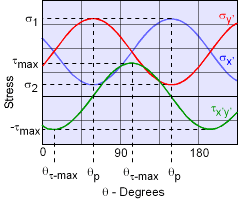
\includegraphics[width=0.8\textwidth]{img/stresses_as_function_of_angle}
            \caption{Stresses as a function of angle}
            \label{fig:stresses_as_function_of_angle-png}
        \end{figure}

        \begin{bbox}[0.85]
            When $\sigma_{x}$ or $\sigma_{y}$ are either max or min, the shear stress
            $\tau_{xy}$ is equal to 0. When shear stress $\tau_{xy}$ is max or min,
            the stresses $\sigma_{x}$ and $\sigma_{y}$ are equal to their average.
        \end{bbox}


\end{itemize}


\section{Moment of Inertia}

From: \href{https://en.wikipedia.org/wiki/Parallel_axis_theorem}{Parallel axis theorem}

\textit{Parallel axis theorem}, also known as \textit{Huygens-Steiner's theorem}
or just \textit{Steiner's theorem} can be used to determine the \textbf{moment of inertia}
or \textbf{second moment of area} of a rigid body about any axis, given the body's
moment of inertia about a parallel axis through the objects center of gravity
and the perpendicular distance between the axes.

Moment of Inertia = \textbf{tensor}.

\begin{itemize}
    \item \textbf{Steiner's share:}

        \begin{equation}
            \mathbf{I}_{ss} = m \times \begin{bmatrix}
                y^{2} + z^{2} & -xy & -xz \\
                -yz & x^{2} + z^{2} & -yz \\
                -zx & -zy & x^{2} + y^{2}
            \end{bmatrix}
        .\end{equation}

        \textbf{Identities for a skew-symmetric matrix}

        In order to compare formulations of the parallel axis theorem using
        skew-symmetric matrices and the tensor formulation, the following
        identities are useful.

        Let $[\mathbf{R}]$ be the skew-symmetric matrix associated with the
        position vector $\mathbf{R} = (x, y, z)$, then the product in
        the inertia matrix becomes:

        \begin{equation}
            -[\mathbf{R}][\mathbf{R}] = \begin{bmatrix}
                0 & -z & y \\
                z & 0 & -x \\
                -y & x & 0
            \end{bmatrix}^{2}
            = \begin{bmatrix}
                y^{2} + z^{2} & -xy & -xz \\
                -yz & x^{2} + z^{2} & -yz \\
                -zx & -zy & x^{2} + y^{2}
            \end{bmatrix}
        .\end{equation}

        This product can be computed using the matrix formed by the outer product
        $[\mathbf{R} \mathbf{R}^{T}]$ using the identity

        \begin{equation}
            \begin{array}{ll}
                 \\
                -[\mathbf{R}]^{2}
                &= |\mathbf{R}|^{2}|\mathbf{E}_{3}| - [\mathbf{R}\mathbf{R}^{T}] \\
                &= \begin{bmatrix}
                    x^{2} + y^{2} + z^{2} & 0 & 0 \\
                    0 & x^{2} + y^{2} + z^{2} & 0 \\
                    0 & 0 & 0
                \end{bmatrix} - \begin{bmatrix}
                    x^{2} & xy & xz \\
                    yx & y^{2} & yz \\
                    zx & zy & z^{2}
                \end{bmatrix}
            \end{array}
        ,\end{equation}

        where $[\mathbf{E}_{3}$ is the $n \times n$  identity matrix.

        Also notice, that

        \begin{equation}
            |\mathbf{R}|^{2} = \mathbf{R} \cdot \mathbf{R} = tr [\mathbf{R}\mathbf{R}^{T}]
        .\end{equation}

        where $tr$ denotes the sum of the diagonal elements of the outer product
        matrix, known as its \textit{trace}.

        To obtain matrix of moments of inertia by rotating about any random
        point $A$ while having the moment of inertia in the center of gravity of
        the object $\mathbf{I}_{COG}$ and the coordinate distance $d = [x, y, z]$
        between the point $A$ and \textbf{COG} we:

        \begin{enumerate}
            \item Compute the moment of inertia relative to point $A$

                 \begin{equation}
                    \mathbf{I}_{A} = \mathbf{I}_{COG} + m \times \mathbf{I}_{SS}^{A \to COG}
                .\end{equation}

            \item Transform the tensor $\mathbf{I}_{A}$ to new rotated coordinate
                system using transformation matrix $\mathbf{T}$:

                \begin{equation}
                    \mathbf{I}_{A}^{'} = \mathbf{T} \times \mathbf{I}_{A} \times \mathbf{T}^{T}
                .\end{equation}

            \item Subtract the \textbf{Steiner's share} relative to new \textbf{COG}

                \begin{equation}
                    \mathbf{I}_{COG}^{'} = \mathbf{I}_{A}^{'} - \mathbf{I}_{SS}^{A' \to COG'}
                .\end{equation}

        \end{enumerate}

\end{itemize}


\newpage

\section{Quaternions}

In mathematics, the quaternion number system extends the complex numbers.
Quaternions were first described by the Irish mathematician William Rowan
Hamilton in 1843 and applied to mechanics in three-dimensional space.
The algebra of quaternions is often denoted by $  \mathbf{H} $
or $ \mathbb{H} $ (for Hamilton).

Although multiplication of quaternions is noncommutative, it gives a definition
of the quotient of two vectors in a three-dimensional space.
Quaternions are generally represented in the form:

\begin{equation}
    a + b \mathbf{i} + c \mathbf{j} + d \mathbf{k}
\end{equation}

where the coefficients $ a, b, c, d $ are \textit{real numbers} and
$ \mathbf{1}, \mathbf{i}, \mathbf{j}, \mathbf{k} $ are \textit{basis vectors} or
\textit{basis elements}.

The Quaterninon multiplication table (left column shows pre-multiplier, top
row shows post-multiplier):

\begin{table}[h!]
    \centering
    \renewcommand{\arraystretch}{1.25}
    % \small
    % \scriptsize
    \scalebox{0.80}{
    \begin{tabular}{||c | c | c | c | c ||}
        \hline
        \hline
        r $ \times $ c  & $ \mathbf{1} $ & $ \quad \mathbf{i} $ & $ \quad \mathbf{j} $ & $ \quad \mathbf{k} $ \\
        \hline
        $ \mathbf{1} $  & $ \mathbf{1} $ & $ \quad \mathbf{i} $ & $ \quad \mathbf{j} $ & $ \quad \mathbf{k} $ \\
        $ \mathbf{i} $  & $ \mathbf{i} $ & $ -\mathbf{1} $ & $ \quad \mathbf{k} $ & $ -\mathbf{j} $ \\
        $ \mathbf{j} $  & $ \mathbf{j} $ & $ -\mathbf{k} $ & $ -\mathbf{1} $ & $ \quad \mathbf{i} $ \\
        $ \mathbf{k} $  & $ \mathbf{k} $ & $ \quad \mathbf{j} $ & $ -\mathbf{i} $ & $ -\mathbf{1} $ \\
        \hline
        \hline
    \end{tabular}}
    \caption{Quaternion multiplication table}
    \label{tab:quat-mult}
\end{table}

also, $ a \mathbf{b} = \mathbf{b} a $ and
$ \mathbf{-b} = (-1) \mathbf{b} $ for $ a \in \mathbb{R}, \quad b = \mathbf{i}, \mathbf{j}, \mathbf{k} $.


\subsection{Quaternion properties}

The following properties apply:

\begin{enumerate}
    \item Addition:

        \begin{eqarray}
            ( a_1 + b_1 \mathbf{i} + c_1 \mathbf{j} + d_1 \mathbf{k} ) +
            ( a_2 + b_2 \mathbf{i} + c_2 \mathbf{j} + d_2 \mathbf{k} ) = \\
            = ( a_1 + a_2 ) + ( b_1 + b_2 ) \mathbf{i} + ( c_1 + c_2 ) \mathbf{j} + ( d_1 + d_2 ) \mathbf{k}
        \end{eqarray}

    \item Component-wise scalar multiplication:

        \begin{equation}
            \lambda ( a + b \mathbf{i} + c \mathbf{j} + d \mathbf{k} ) =
            \lambda a + (\lambda b) \mathbf{i} + (\lambda c) \mathbf{j} + (\lambda d) \mathbf{k}
        \end{equation}

    \item Multiplication of basis elements (the revelation of Hamilton in 1943):

        \begin{eqarray}
            \mathbf{i}^2 = \mathbf{j}^2 = \mathbf{k}^2 &= -1 \\
            \mathbf{i} \mathbf{j} \mathbf{k} &= -1
        \end{eqarray}

    \item Multiplicative identity:

        \begin{eqarray}
            \mathbf{i} 1 = \quad 1 \mathbf{i} &= \quad \mathbf{i} \\
            \mathbf{j} 1 = \quad 1 \mathbf{j} &= \quad \mathbf{j} \\
            \mathbf{k} 1 = \quad 1 \mathbf{k} &= \quad \mathbf{k}
        \end{eqarray}

    \item Products of basis elements:

        \begin{eqarray}
            \mathbf{i} \mathbf{j} = -\mathbf{j} \mathbf{i} &= \quad \mathbf{k} \\
            \mathbf{j} \mathbf{k} = -\mathbf{k} \mathbf{j} &= \quad \mathbf{i} \\
            \mathbf{k} \mathbf{i} = -\mathbf{i} \mathbf{k} &= \quad \mathbf{j}
        \end{eqarray}

    \item Inverse:

        \begin{equation}
            (a + b \mathbf{i} + c \mathbf{j} + d \mathbf{k})^{-1}
            = \frac{1} {a^2 + b^2 + c^3 + d^2} (a - b \mathbf{i} - c \mathbf{j} - d \mathbf{k})
        \end{equation}

    \item Product of two \textbf{quaternions} (also called the \textbf{Hamilton product})
        is determined by the products of the basis elements and the \textbf{distributive} law:

        \begin{equation}
            ( a_1 + b_1 \mathbf{i} + c_1 \mathbf{j} + d_1 \mathbf{k} ) \times
            ( a_2 + b_2 \mathbf{i} + c_2 \mathbf{j} + d_2 \mathbf{k} ) = \\
        \end{equation}

        \begin{eqarray}
            = & a_1 a_2 \quad &+& a_1 b_2 \mathbf{i} &+& a_1 c_2 \mathbf{j} &+& a_1 d_2 \mathbf{k} \\
            + & b_1 a_2 \mathbf{i} &+& b_1 b_2 \mathbf{i}^2 &+& b_1 c_2 \mathbf{i} \mathbf{j} &+& b_1 d_2 \mathbf{i} \mathbf{k} \\
            + & c_1 a_2 \mathbf{j} &+& c_1 b_2 \mathbf{i} \mathbf{j} &+& c_1 c_2 \mathbf{j}^2 &+& c_1 d_2 \mathbf{j} \mathbf{k} \\
            + & d_1 a_2 \mathbf{k} &+& d_1 b_2 \mathbf{i} \mathbf{k} &+& d_1 c_2 \mathbf{j} \mathbf{k} &+& d_1 d_2 \mathbf{k}^2
        \end{eqarray}

        \begin{eqarray}
            = & a_1 a_2 \quad &-& b_1 b_2 &-& c_1 c_2 &-& d_1 d_2 \\
            + & ( a_1 b_2 &+& b_1 a_2 &+& c_1 d_2 &-& d_1 c_2 ) \times \mathbf{i} \\
            + & ( a_1 c_2 &-& b_1 d_2 &+& c_1 a_2 &+& d_1 b_2 ) \times \mathbf{j} \\
            + & ( a_1 d_2 &+& b_1 c_2 &-& c_1 b_2 &+& d_1 a_2 ) \times \mathbf{k}
        \end{eqarray}

\end{enumerate}


\subsection{Scalar and vector parts}

A quaternion of the form $ a + 0 \mathbf{i} + 0 \mathbf{j} + 0 \mathbf{k} $,
where $ a $ is a real number, is called \textbf{scalar}, and a quaternion of the form
$ 0 + b \mathbf{i} + c \mathbf{j} + d \mathbf{k} $ where $ b $, $ c $ and $ d $
are real numbers, and at least on of $ b $, $ c $ or $ d $ is nonzero, is called
a \textbf{vector quaternion}. If $ a + b \mathbf{i} + c \mathbf{j} + d \mathbf{k} $
is any quaternion, then $ a $ is called its \textbf{scalar part} and
$ b \mathbf{i} + c \mathbf{j} + d \mathbf{k} $ is called its \textbf{vector part}.
Although every quaternion can be viewed as a vector in a four-dimensional
vector space, it is common to refer to the \textbf{vector} part as vectors in
three-dimensional space.

Hamilton also called vector quaternions \textbf{right quaternions} and real
numbers (considered as quaternions with zero vector part) \textbf{scalar quaternions}.

If a quaternion is divided up into a scalar and a vector part, that is,

\begin{equation}
    \mathbf{q} = (r, \vec{v}), \mathbf{q} \in \mathbb{H}, r \in \mathbb{R}, \vec{v} \in \mathbb{R}^3
\end{equation}

then the formulas for \textbf{addition}, \textbf{multiplication}
and \textbf{multiplicative inverse} are:

\begin{equation}
    (r_1, \vec{v}_1) + (r_2, \vec{v}_2) = (r_1 + r_2, \vec{v}_1 + \vec{v}_2 )
\end{equation}

\begin{equation}
    (r_1, \vec{v}_1) \times (r_2, \vec{v}_2) = (r_1 r_2 - \vec{v}_1 \cdot \vec{v}_2, r_1 \vec{v}_2 + r_2 \vec{v}_1 + \vec{v}_1 \times \vec{v}_2)
\end{equation}

\begin{equation}
    (r, \vec{v})^{-1} =
    \left(
        \frac{r} {r^2 + \vec{v} \cdot \vec{v}},
        \frac{-\vec{v}} {r^2 + \vec{v} \cdot \vec{v}}
    \right)
\end{equation}


\subsection{Conjugation, the norm and reciprocal}

Conjugation of quaternions is analogous to conjugation of complex numbers.
To define it, let $ \mathbf{q} = a + b \mathbf{i} + c \mathbf{j} + d \mathbf{k} $
be a quaternion. The \textbf{conjugate} of $ \mathbf{q} $ is the quaternion
$ \mathbf{q}^{*} = a - b \mathbf{i} - c \mathbf{j} - d \mathbf{k} $.
It is denoted by $ \mathbf{q}^{*} $, $ \mathbf{q}^{t} $ or $ \bar{\mathbf{q}} $.

\textbf{Conjugation} is \textbf{involution}, meaning that it is its own inverse,
so \textbf{conjugating} an element \textbf{twice} returns the original element.
The \textbf{conjugate} of a \textbf{product} of two quaternions is the product of the
conjugates in the \textbf{reverse order}. That is, if $ \mathbf{p} $ and
$ \mathbf{q} $ are quaterninos, then:

\begin{equation}
    ( \mathbf{p} \mathbf{q} )^{*} = \mathbf{q}^{*} \mathbf{p}^{*}
\end{equation}


The conjugation of a quaternion, in stark contrast to the complex setting, can be
expressed with multiplication and addition of quaternions:

\begin{equation}
    \mathbf{q}^{*} = -\frac{1}{2} (\mathbf{q}
    + \mathbf{i} \mathbf{q} \mathbf{i}
    + \mathbf{j} \mathbf{q} \mathbf{j}
    + \mathbf{k} \mathbf{q} \mathbf{i} )
\end{equation}


Conjugation can be used to extract the \textbf{scalar} and \textbf{vector} part of a
quaternion. The \textbf{scalar} part of $ \mathbf{q} $ is:

\begin{equation}
    r_q = \frac{1}{2} ( \mathbf{q} + \mathbf{q}^{*} )
\end{equation}

The \textbf{vector} part of $ \mathbf{q} $ is:

\begin{equation}
    \vec{v}_q = \frac{1}{2} ( \mathbf{q} - \mathbf{q}^{*} )
\end{equation}

The \textbf{square root} of the product of a quaternion with its conjugate is called
its \textbf{norm} and is denoted $ \| q \| $ (Hamilton called this quantity
the \textbf{tensor} of $ \mathbf{q} $).

\begin{equation}
    \| \mathbf{q} \| = \sqrt{ \mathbf{q}^{*} \mathbf{q} }
    = \sqrt{ \mathbf{q} \mathbf{q}^{*} }
    = \sqrt{ a^2 + b^2 + c^2 + d^2 } \in \mathbb{R} \ge 0
\end{equation}

This is always a non-negative, real number and is the same as the Euclidean norm
on $ \mathbb{H} $ considered as the vector space $ \mathbb{R}^4 $. Multiplying
a quaternion by a real number scales its norm by the absolute value of the number.
That is, if $ \alpha \in \mathbb{R} $ then:

\begin{equation}
    \norm{\alpha \m{q}} = \abs{\alpha} \norm{\m{q}}
\end{equation}

The norm is \textbf{multiplicative}, meaning that:

\begin{equation}
    \norm{\m{p} \m{q}} = \norm{\m{p}} \norm{\m{q}}
\end{equation}

for any two quaternion $ \m{p} $ and $ \m{q} $. Multiplicativity is a consequence of the
formula for the conjugate of a product. Alternatively it follows fom the identity

\begin{equation}
    det \left( \begin{matrix}
            a + i b & id + c \\
            id - c & a - ib
          \end{matrix} \right) = a^2 + b^2 + c^2 + d^2
\end{equation}

(where $ i $ denotes the usual imaginary unit) and hence from the multiplicative
property of determinants of square matrices.

This norm makes it possible to define the \textbf{distance} $ d(\m{p},\m{q}) $
between $ \m{p} $ and $ \m{q} $ as the norm of their difference:

\begin{equation}
    d(\m{p},\m{q}) = \norm{\m{p} - \m{q}}
\end{equation}

This makes $ \mathbb{H} $ a \textbf{metric space}. Addition and multiplication are
\textbf{continuous} in regard to the associated metric topology. This
follows exactly the same proof as for the real numbers $ \mathbb{R} $ from the
fact that $ \mathbb{H} $ is a \textbf{normed algebra}.


\subsection{Unit quaternion (or versor)}

A \textbf{unit quaternion} is a quaternion of norm one. Dividing a nonzero quaternion
$ \m{q} $ by its norm produces a unit quaternion $ \m{Uq} $ called the \textbf{versor}
of $ \m{q} $:

\begin{equation}
    \m{Uq} = \frac{\m{q}} {\norm{\m{q}}}
\end{equation}

Every nonzero quaternion has a unique \textbf{polar decomposition}
$ \m{q} = \norm{\m{q}} \cdot \m{Uq} $, while the zero quaternion can be formed
from any unit quaternion.

Using conjugation and the norm makes it possible to define the \textbf{reciprocal}
of a nonzero quaternion. The product of a quaternion with its reciprocal should
be equal 1, and the considerations above imply that the product of $ \m{q} $ and
$ \m{q}^{*} / \norm{\m{q}}^2 $ is 1 (for any order fo multiplication). So the
\textbf{reciprocal} of $ \m{q} $ is defined to be:

\begin{equation}
    \m{q}^{-1} = \frac{\m{q}^{*}}{\norm{\m{q}}^2}
\end{equation}

Since the multiplication is non-commutative, the quotient quantities
$ \m{p} \m{q}^{-1} $ or $ \m{q}^{-1} \m{p} $ are different (except if $ \m{p} $
and $ \m{q} $ are scalar multiples of each other or if one is a scalar).
The notation $ \frac{p}{q} $ is ambiguous and \textbf{should not be used}.



\subsection{Quaternions and three-dimensional geometry}

The vector part of a quaternion can be interpreted as a coordinate vector
in $ \mathbb{R}^3 $, therefore the algebraic operations fo the quaternions reflect
the geometry of $ \mathbb{R}^3 $. Operations such as the vector dot and cross
products can be defined in terms of quaternions and thei makes it possible to apply
quaternion techniques wherever spatial vectors arise. A useful application of quaternions
has been to interpolate the orientations of key-frames in computer graphics.

For the remainder of this section, $ \m{i} $, $ \m{j} $ and $ \m{k} $ wil denote
both the three imaginary basis vectors of $ \mathbb{H} $ and a basis for $ \mathbb{R}^3 $.
Replacing $ \m{i} $ by $ -\m{i} $, $ \m{j} $ by $ -\m{j} $ and $ \m{k} $ by $ -\m{k} $
sends a vector to its \textbf{additive inverse}, so the additive inverse of a vector
is the same as its conjugate as a quaternion. For this reason, conjugation
is sometimes called the \textbf{spatial inverse}.

For two vector quaternions $ \m{p} = b_1 \m{i} + c_1 \m{j} + d_1 \m{k} $ and
$ \m{q} = b_2 \m{i} + c_2 \m{j} + d_2 \m{k} $ their \textbf{dot product}, by
analogy to vectors in $ \mathbb{R}^3 $, is:

\begin{equation}
    \m{p} \cdot \m{q} = b_1 b_2 + c_1 c_2 + d_1 d_2
\end{equation}

It can also be expressed ina a component-free manner as:

\begin{equation}
    \m{p} \cdot \m{q} = \frac{1}{2} (\m{p}^{*} \m{q} + \m{q}^{*} \m{p})
    = \frac{1}{2} (\m{p} \m{q}^{*} + \m{q} \m{p}^{*})
\end{equation}

This is equal to the scalar parts of the products $ \m{p} \m{q}^{*} $,
$ \m{q} \m{p}^{*} $, $ \m{p}^{*} \m{q} $ and $ \m{q}^{*} \m{p} $. Note that their
vector parts are different.

The \textbf{cross product} of $ \m{p} $ and $ \m{q} $ relative to the orientation
determined by the ordered basis $ \m{i} $, $ \m{j} $ and $ \m{k} $ is:

\begin{equation}
    \m{p} \times \m{q} = (c_1 d_2 - d_1 c_2) \m{i}
    + (d_1 b_2 - b_1 d_2) \m{j} + (b_1 c_2 - c_1 b_2) \m{k}
\end{equation}

(The orientation is necessary to determine the sign.) This is equal to the vector
part of the product $ \m{p} \m{q} $ (as quaternions), as well as the vector part of
$ -\m{q}^{*} \m{p}^{*} $. It also has the formula:

\begin{equation}
    \m{p} \times \m{q} = \frac{1}{2} ( \m{p} \m{q} - \m{q} \m{p})
\end{equation}

For the \textbf{commutator}, $ [\m{p}, \m{q}] = \m{p} \m{q} - \m{q} \m{p} $ of two
vector quaternions one obtains:

\begin{equation}
    [\m{p}, \m{q}] = 2 \m{p} \times \m{q}
\end{equation}

In general, let $ \m{p} $ and $ \m{q} $ be quaternions and write:

\begin{eqarray}
    \m{p} &= \m{p}_s + \m{p}_v \\
    \m{q} &= \m{q}_s + \m{q}_v
\end{eqarray}

where $ \m{p}_s $ and $ \m{q}_s $ are the scalar parts, and $ \m{p}_v $ and $ \m{q}_v $.
Then we have the formula:

\begin{equation}
    \m{p} \m{q} = (\m{p} \m{q})_s + (\m{p} \m{q})_v
    = (\m{p}_s \m{q}_s -  \m{p}_v \cdot \m{q}_v )
    + (\m{p}_s \m{q}_v + \m{q}_s \m{p}_v + \m{p}_v \times \m{q}_v)
\end{equation}

This shows that the noncommutativity of quaternion multiplication comes from the
multiplication of vector quaternions. It also shows that two quaternions commute
if and only if their vector parts are collinear. \textbf{Hamilton} showed that
this product computes the third vertex of spherical triangle from two given
vertices and their associated arc-lengths, which is also an algebra of points
in \textbf{Elliptic geometry}.

\textbf{Unit quaternions} can be identified with rotations in $ \mathbb{R}^3 $
and were called \textbf{versors} by \textbf{Hamilton}.


\subsection{Matrix representations}

Just as complex numbers can be \textbf{represented as matrices}, co can be quaternions.
There are \textit{at least} two ways to represent quaternions as matrices in
such a way that quaternion \textbf{addition} and \textbf{multiplication} correspond
to the matrix addition and multiplication.

The quaternion $ a + b \m{i} + c \m{j} + d \m{k} $ can be represented:

\begin{enumerate}
    \item as a $ 2 \times 2 $ complex matrix:

        \begin{equation}
            \begin{bmatrix}
                \q a + b i  &  c + d i \\
                -c + d i  & a - bi
            \end{bmatrix}
        \end{equation}

        This representation has the following properties:

        \begin{itemize}
            \item Constraining any two of $ b $, $ c $ and $ d $ to zero produces
                a representation fo complex numbers. For example, setting $ c = d = 0 $
                produces a diagonal complex matrix representation of complex numbers,
                and setting $ b = d = 0 $ produces a real matrix representation.

            \item The \textbf{norm} of a quaternion (the square root of the product
                with its conjugate, as with complex numbers) is the square root
                of the \textbf{determinant} of the corresponding matrix.

            \item The \textbf{conjugate} of a quaternion corresponds to the
                \textbf{conjugate transpose} of the matrix.

            \item There is a strong relation between quaternion units and
                \textbf{Pauli matrices} (these are needed to describe the
                \textit{spin in quantum mechanics}). Obtain the eight quaternion unit matrices
                by taking $ a $, $ b $, $ c $ and $ d $, set three of them to zero
                and the fourth to $ 1 $ or $ -1 $. Multiplying any two Pauli matrices
                always yields a quaternion unit matrix, all of them except for $ -1 $.
                One obtains $ -1 $ via the last equality:

                \begin{eqarray}
                    \m{i}^2 = \m{j}^2 = \m{k}^2 = \m{i} \m{j} \m {k} = -1 \\
                    i j k = \sigma_1 \sigma_2 \sigma_3 \sigma_1 \sigma_2 \sigma_3 = -1
                \end{eqarray}

        \end{itemize}

    \item Using $ 4 \times 4 $ real matrix the same quaternion can be written as:

        \begin{eqarray}
            \begin{bmatrix}
                a & -b & -c  & -d \\
                b & \q a & -d & \q c \\
                c & \q d & \q a & -b \\
                d & -c & \q b & \q a \\
            \end{bmatrix}
            &= a \begin{bmatrix}
                1 & \q 0 & \q 0 & \q 0 \\
                0 & \q 1 & \q 0 & \q 0 \\
                0 & \q 0 & \q 1 & \q 0 \\
                0 & \q 0 & \q 0 & \q 1
            \end{bmatrix} \\
            &+ b \begin{bmatrix}
                0 &   -1 & \q 0 & \q 0 \\
                1 & \q 0 & \q 0 & \q 0 \\
                0 & \q 0 & \q 0 &   -1 \\
                0 & \q 0 & \q 1 & \q 0
            \end{bmatrix} \\
            &+ c \begin{bmatrix}
                0 & \q 0 &   -1 & \q 0 \\
                0 & \q 0 & \q 0 & \q 1 \\
                1 & \q 0 & \q 0 & \q 0 \\
                0 &   -1 & \q 0 & \q 0
            \end{bmatrix} \\
            &+ d \begin{bmatrix}
                0 & \q 0 & \q 0 &   -1 \\
                0 & \q 0 &   -1 & \q 0 \\
                0 & \q 1 & \q 0 & \q 0 \\
                1 & \q 0 & \q 0 & \q 0
            \end{bmatrix} \\
        \end{eqarray}

        However the representation above is not unique. For example, the same quaternion
        can be also represented as:

        \begin{eqarray}
            \begin{bmatrix}
                \q a & \q d &   -b  &  -c \\
                  -d & \q a & \q c &   -b \\
                \q b &   -c & \q a &   -d \\
                \q c & \q b & \q d & \q a \\
            \end{bmatrix}
            &= a \begin{bmatrix}
                \q 1 & \q 0 & \q 0 & \q 0 \\
                \q 0 & \q 1 & \q 0 & \q 0 \\
                \q 0 & \q 0 & \q 1 & \q 0 \\
                \q 0 & \q 0 & \q 0 & \q 1
            \end{bmatrix} \\
            &+ b \begin{bmatrix}
                \q 0 & \q 0 &   -1 & \q 0 \\
                \q 0 & \q 0 & \q 0 &   -1 \\
                \q 1 & \q 0 & \q 0 & \q 0 \\
                \q 0 & \q 1 & \q 0 & \q 0
            \end{bmatrix} \\
            &+ c \begin{bmatrix}
                \q 0 & \q 0 & \q 0 &   -1 \\
                \q 0 & \q 0 & \q 1 & \q 0 \\
                \q 0 &   -1 & \q 0 & \q 0 \\
                \q 1 & \q 0 & \q 0 & \q 0
            \end{bmatrix} \\
            &+ d \begin{bmatrix}
                \q 0 & \q 1 & \q 0 & \q 0 \\
                  -1 & \q 0 & \q 0 & \q 0 \\
                \q 0 & \q 0 & \q 0 &   -1 \\
                \q 0 & \q 0 & \q 1 & \q 0
            \end{bmatrix} \\
        \end{eqarray}

        There exist 48 distinct matrix representations of thei form in which one of the
        matrices represents the scalar part and the other three are all skew-symmetric.

\end{enumerate}


\subsection{Exponential, logarithm and power functions}

Given a quaternion:

\begin{equation}
    \m{q} = a + b \m{i} + c \m{j} + d \m{k} = r + \vec{\m{v}}
\end{equation}

\begin{enumerate}
    \item the exponential is computed as

        \begin{equation}
            \exp(\m{q}) = \sum_{n=0}^{\infty} \frac{\m{q}^n}{n!}
            = e^a \left( \cos \norm{\vec{\m{v}}}
            + \frac{\vec{\m{v}}}{\norm{\vec{\m{v}}}} \sin \norm{\vec{\m{v}}} \right)
        \end{equation}

    \item the logarithm is:

        \begin{equation}
            \ln(\m{q}) = \ln \norm{\m{q}}
            + \frac{\vec{\m{v}}}{\norm{\vec{\m{v}}}}
            \arccos \frac{r}{\norm{\m{q}}}
        \end{equation}

    \item it follows that the polar decomposition of a quaternion may be written

        \begin{equation}
            \m{q} = \norm{\m{q}}e^{\hat{\m{n}} \varphi} = \norm{\m{q}}
            \left( \cos(\varphi) + \hat{\m{n}} \sin(\varphi) \right)
        \end{equation}

        where the angle $ \varphi $ is defined as

        \begin{equation}
            r = \norm{\m{q}} \cos(\varphi)
        \end{equation}

        and the unit vecotr $ \hat{\m{n}} $ is defined by

        \begin{equation}
            \vec{\m{v}} = \hat{\m{n}} \norm{\vec{\m{v}}}
            = \hat{\m{n}} \norm{\m{q}} \sin(\varphi)
        \end{equation}

        Any unit quaternion may be expressed in polar form as:

        \begin{equation}
            \m{q} = \exp(\hat{\m{n}} \varphi)
        \end{equation}

    \item The power of a quaternion raised to an arbitrary (real) exponend $ x $ is
        given by:

        \begin{equation}
            \m{q}^x = \norm{\m{q}}^x e^{\hat{\m{n}} x \varphi}
            = \norm{\m{q}}^x
            \left(\cos(x \varphi) + \hat{\m{n}} \sin(x \varphi) \right)
        \end{equation}

\end{enumerate}


\subsection{Quaternions used for coordinate transformation}

One can think of \textbf{quaternions} as a stored information about coordinate
mapping from one space to another. We can split arbitrary \textbf{quaternion}\\
$ \mathbf{q} = a + b \mathbf{i} + c \mathbf{j} + d \mathbf{k} $ into \textbf{two} parts:

\begin{enumerate}
    \item a \textbf{real} part $ r = a $ and

    \item a \textbf{vector} part $ \mathbf{v} = \left[ b, c, d \right] $.

\end{enumerate}

Next, if we \textbf{impose} restrictions on such \textbf{quaternions} that:

\begin{enumerate}
    \item the \textbf{real} part must satisfy: $ r \in \left< -\pi; \pi \right> $

    \item the \textbf{vector} part must have \textbf{unit} length:
        $ | \textbf{v} | = \sqrt{b^2 + c^2 + d^2} = 0 $

\end{enumerate}

Then, if one thinks of the complex numbers $ \mathbf{i} $, $ \mathbf{j} $ and $ \mathbf{k} $
as of basis vectors of cartesian system $ \mathbf{x} $, $ \mathbf{y} $ and $ \mathbf{z} $, where

\begin{eqarray}
    \mathbf{x} &= \left[ 1.0, 0.0, 0.0 \right] \\
    \mathbf{y} &= \left[ 0.0, 1.0, 0.0 \right] \\
    \mathbf{z} &= \left[ 0.0, 0.0, 1.0 \right]
\end{eqarray}

the quaternion multiplication table \ref{tab:quat-mult} makes sense in relation to \textbf{vector cross product}:

\begin{table}[h!]
    \centering
    \renewcommand{\arraystretch}{1.25}
    % \small
    % \scriptsize
    \scalebox{0.80}{
    \begin{tabular}{||c | c | c | c | c ||}
        \hline
        \hline
        r $ \times $ c  & $ \mathbf{1} $ & $ \quad \mathbf{x} $ & $ \quad \mathbf{y} $ & $ \quad \mathbf{z} $ \\
        \hline
        $ \mathbf{1} $  & $ \mathbf{1} $ & $ \quad \mathbf{x} $ & $ \quad \mathbf{y} $ & $ \quad \mathbf{z} $ \\
        $ \mathbf{x} $  & $ \mathbf{x} $ & $ -\mathbf{1} $ & $ \quad \mathbf{z} $ & $ -\mathbf{y} $ \\
        $ \mathbf{y} $  & $ \mathbf{y} $ & $ -\mathbf{z} $ & $ -\mathbf{1} $ & $ \quad \mathbf{x} $ \\
        $ \mathbf{z} $  & $ \mathbf{z} $ & $ \quad \mathbf{y} $ & $ -\mathbf{x} $ & $ -\mathbf{1} $ \\
        \hline
        \hline
    \end{tabular}}
    \caption{Quaternion cartesian base vectors multiplication table}
    \label{tab:quat-mult-cart}
\end{table}


\begin{bbox}

    In 3-dimensional space, according to the \textbf{Euler's rotation theorem}, any
    rotation or a sequence of rotations of a rigid body or coordinate system about a fixed
    point is equivalent to a single rotation by a given angle $ \theta $ about
    a fixed axis (called the \textit{Euler axis}) that runs through the fixed point.
    The Euler axis is typically represented by a \textbf{unit vector} $ \vec{\m{u}} $.
    Therefore, any rotation in three dimensions can be represented as via
    a \textbf{vector} $ \vec{\m{u}} $ and and angle $ \theta $.

    Quaternions give a simple way to encode this \textbf{axis-angle} representation
    using four real numbers and can be used to apply (calculate) the corresponding
    rotation to a \textbf{position vector} $ [x, y, z] $, representing a point
    relative to the origin in $ \mathbb{R}^3 $.

\end{bbox}

Euclidean vectors such as $ [a_x, a_y, a_z] $ can be rewritten as
$ a_x \m{i} + a_y \m{j} + a_z \m{k} $, where $ \m{i} $, $ \m{j} $ and $ \m{k} $ are
unit vectors representing the three \textbf{Cartesian axies} (traditionally
$ \m{x} $, $ \m{y} $ and $ \m{z} $) and also obey the \textbf{multiplication} rules
of the fundamental quaternion units by interpreting the Euclidean vector
$ [a_x, a_y, a_z] $ as the vector part of the pure quaternion
$ (0, a_x, a_y, a_z) $.

A rotation angle $ \theta $ around the axis defined by the unit vector

\begin{equation}
    \vec{\m{u}} = (u_x, u_y, u_z) = u_x \m{i} + u_y \m{j} + u_z \m{k}
\end{equation}

can be represented by \textbf{conjugation} by a unit quaternion $ \m{q} $.

Since the quaternion product

\begin{equation}
    (0 + u_x \m{i} + u_y \m{j} + u_z \m{k})
    (0 - u_x \m{i} - u_y \m{j} - u_z \m{k}) = -1
\end{equation}

using \textbf{Taylor series} of the exponential function, the extension
of the Euler's formula results in:

\begin{eqarray}
    \m{q} &= e^{\frac{\theta}{2}(u_x \m{i} + u_y \m{j} + u_z \m{k})} \\
          &= \cos \frac{\theta}{2} + \left( u_x \m{i} + u_y \m{j} + u_z \m{k} \right)
          \sin \frac{\theta}{2} \\
          &= \cos \frac{\theta}{2} + \vec{\m{u}} \sin \frac{\theta}{2}
\end{eqarray}

It can be shown that the desired rotation can be applied to an ordinary vector

\begin{equation}
    \m{p} = (p_x, p_y, p_z) = p_x \m{i} + p_y \m{j} + p_z \m{k}
\end{equation}

in 3-dimensional space, considered as the vector part of the pure quaternion $ \m{p}' $,
by evaluating the \textbf{conjugation} of $ \m{p}' $ by $ \m{q} $, given by:

\begin{eqarray}
    L(\m{p}') &:= \m{q} \m{p}' \m{q}^{-1} \\
    r &= \left(\cos^2 \frac{\theta}{2} - \norm{\m{u}}^2 \right)
    + 2 ( \m{u} \cdot \m{p}) \m{u}
    + 2 \cos \frac{\theta}{2} (\m{u} \times \m{p})
\end{eqarray}

using the \textbf{Hamilton product} where the vector part of the pute quaternion
$ L(\m{p}') = (0, r_x, r_y, r_z) $ is the new position vector after the rotation.
In a programmatic implementation \textbf{the conjugation} is achieved by constructing
a pure quaternion whise vector part is $ \m{p} $, and then performing the quaternion
conjugation. The vector part of the resulting pure quaternion is the desired
vector $ \m{r} $. Clearly $ L $ provides a linear transformation of the quaternion
space to itself, also, since $ \m{q} $ is unitary, the transformation is an
isometry. Also $ L(\m{q}) = \m{q} $ ans so $ L $ leaves vectors parallel to
$ \m{q} $ invariant. So, by decomposing $ \m{p} $ as a vector parallel to the
vector part $ (u_x, u_y, u_z) \sin \frac{\theta}{2} $ of $ \m{q} $ and a vector
normal to the vector part of $ \m{q} $ and showing that the application of
$ L $ to the normal component of $ \m{p} $ rotates it, the claim is shown.

So let $ \m{n} $ be the component of $ \m{p} $ orthogonal to the vector part
of $ \m{q} $ and let $ \m{n}_T = \m{n} \times \m{u} $. It turns out that the
vector part of $ L(0, \m{n}) $ is given by:

\begin{equation}
    \left(\cos^2 \frac{\theta}{2} - \sin^2 \frac{\theta}{2} \right) \m{n}
    + 2 \left(\cos^2 \frac{\theta}{2} \sin^2 \frac{\theta}{2} \right) \m{n}_T
    = \cos \theta \m{n} + \sin \theta \m{n}_T
\end{equation}

A geometric fact independent of quaternion is the existence of \textbf{two-to-one}
mapping from physical rotations to rotational transformation matrices.

If $ 0 \le \theta \le 2 \pi $, a physical rotaion about $ \vec{\m{u}} $ by
$ \theta $ and a physical rotation about $ -\vec{\m{u}} $ by $ 2 \pi - \theta $
both achieve the \textbf{same final orientation} by disjoint paths through
intermediate orientations.

By inserting those vectors and angles into the formula for $ \m{q} $ above,
one findes that if $ \m{q} $ represents the first rotation, $ -\m{q} $
represents the second rotation. This is a geometric proof that conjugation
by $ \m{q} $ and by $ -\m{q} $ must produce the same rotational transformation
matrix. That fact is confirmed algebraically by noting that the conjugation is
quadratic in $ \m{q} $, so the sign of $ \m{q} $ cancels, and does not affect
the result.

If both rotations are a half-turn $ (\theta = \pi) $, both $ \m{q} $ and
$ -\m{q} $ will have real coordinate equal to zero. Otherwise, one will have a positive
real part, representing a rotation by an angle less than $ \pi $, and the other
will have a negative real part, representing a rotation by an angle greater than $ \pi $.

Mathemativally, this operation carries the set of all "pure" quaterninos
$ \m{p} $ (thise with real part equal to zero) - which consitute a 3-dimensional
space among the quaternions - into itself, by the desired rotation about the axis
$ \m{u} $, by the angle $ \theta $.

The rotation is \textbf{clockwise} if our line of sight points in the same direction
as $ \vec{\m{u}} $.

In the instance that $ \m{q} $ is a \textbf{unit quaternion} and

\begin{equation}
    \m{q}^{-1} = e^{-\frac{\theta}{2} ( u_x \m{i} + u_y \m{j} + u_z \m{k} )}
    = \cos \frac{\theta}{2} - ( u_x \m{i} + u_y \m{j} + u_z \m{k} ) \sin \frac{\theta}{2}
\end{equation}

It follows that conjugation by the product of two quaternions is the composition of
conjugations by these quaternions. If $ \m{p} $ and $ \m{q} $ are unit quaternions,
then conjugation (\textbf{rotation}) by $ \m{p} \m{q} $ is:

\begin{equation}
    \m{p} \m{q} \vec{\m{v}} ( \m{p} \m{q} )^{-1}
    = \m{p} \m{q} \vec{\m{v}} \m{q}^{-1} \m{p}^{-1}
    = \m{p} ( \m{q} \vec{\m{v}} \m{q}^{-1} ) \m{p}^{-1}
\end{equation}

which is \textbf{the same} as conjugating (\textbf{rotating}) by $ \m{q} $ and
then by $ \m{p} $. The scalar component of the result is \textbf{necessarily zero}.

The quaternion \textbf{inverse} of a rotation is the opposite rotation, since

\begin{equation}
    \m{q}^{-1} (\m{q} \vec{\m{v}} \m{q}^{-1} ) \m{q} = \vec{\m{v}}
\end{equation}

The square of a quaternion rotation is a rotation by twice the angle around the same axis.



